\documentclass[11pt,a4paper,DIV=12]{scrartcl}
\PassOptionsToPackage{dvipsnames}{xcolor}
\usepackage{multicol}
\makeatletter
\def\input@path{{../../../}}
\makeatother

\usepackage[sexy]{evan}

\makeatletter
\newtheoremstyle{problemstyle}
  {8pt} 
  {8pt} 
  {\normalfont} 
  {} 
  {\color{blue!40!black}\bfseries} 
  {} 
  {0.5em} 
  {\thmnumber{#2}.\thmnote{ (\small #3)}} 

\let\problem\@undefined
\let\endproblem\@undefined
\let\c@problem\@undefined
\let\theproblem\@undefined
\makeatother

\makeatletter
\newtheoremstyle{answerstyle}
  {8pt} 
  {8pt} 
  {\normalfont} 
  {}
  {\color{blue!40!black}\bfseries} 
  {} 
  {\newline} 
  {\thmnumber{#2}. \thmnote{\fbox{\bfseries #3}}} 

\let\answer\@undefined
\let\endanswer\@undefined
\let\c@answer\@undefined
\let\theanswer\@undefined
\makeatother

\newcommand\answerbox{%%
\vspace*{0.5cm}%
\noindent\textbf{\textsf{Jawab}}: \fbox{\rule{14cm}{0pt}\rule[-0.2ex]{0pt}{1.9ex}}}

\theoremstyle{problemstyle}
\newtheorem{problem}{}
\theoremstyle{answerstyle}
\newtheorem{answer}{}

\newenvironment{choices}[1][5]{%
  \begin{multicols}{#1}%
  \begin{enumerate}[label=(\Alph*)]%
}{%
  \end{enumerate}%
  \end{multicols}%
}

\begin{document}
\title{Tryout 2 Pembinaan OSK Matematika}
\author{MAN 1 Pasuruan}
\date{Mei 2025}
\maketitle
\noindent\textbf{Petunjuk pengerjaan:}
\begin{itemize}
  \item Waktu pengerjaan adalah 120 menit.
  \item Terdapat 20 soal yang terdiri dari 10 soal pilihan ganda dan 10 soal kemampuan isian singkat.
  \item Nilai soal pilihan ganda adalah {\color{green!70!black}$B=+1$}, {\color{red}$S=0$}, $K=0$.
  \item Nilai soal isian singkat adalah {\color{green!70!black}$B=+4$}, {\color{red}$S=0$}, $K=0$.
  \item Gunakan bolpoin untuk menulis jawaban, dan coretlah jawaban yang salah.
\end{itemize}

\section*{Pilihan Ganda}
\begin{problem}
  Berapa banyak dari sepuluh suku pertama barisan
  \[
    121,11211,1112111,\dots
  \]
  yang merupakan bilangan prima?

  \begin{choices}
    \item $0$
    \item $1$
    \item $2$
    \item $3$
    \item $4$
  \end{choices}
  %KJ : A
\end{problem}
\begin{problem}
  Salah satu dari bilangan berikut tidak habis dibagi oleh bilangan prima mana pun yang kurang dari \(10\).
  Bilangan yang manakah itu?

  \begin{choices}
    \item $2^{606}-1$
    \item $2^{606}+1$
    \item $2^{607}-1$
    \item $2^{607}+1$
    \item $2^{607}+3^{607}$
  \end{choices}
  %KJ : C
\end{problem}
\begin{problem}
  Barisan \(a_0,a_1,a_2,\dots\) adalah suatu barisan aritmetika naik ketat yang terdiri dari bilangan bulat positif dan memenuhi
  \[
    2^{a_7}=2^{27}\cdot a_7.
  \]

  Berapakah nilai minimum yang mungkin dari \(a_2\)?

  \begin{choices}
    \item $8$
    \item $12$
    \item $16$
    \item $17$
    \item $22$
  \end{choices}
  %KJ : B
\end{problem}
\begin{problem}
  Misalkan \(a,b,c,\) dan \(d\) adalah bilangan bulat positif yang memenuhi semua relasi berikut:
  \[
    abcd=2^6\cdot 3^9\cdot 5^7
  \]
  \[
    \operatorname{lcm}(a,b)=2^3\cdot 3^2\cdot 5^3
  \]
  \[
    \operatorname{lcm}(a,c)=2^3\cdot 3^3\cdot 5^3
  \]
  \[
    \operatorname{lcm}(a,d)=2^3\cdot 3^3\cdot 5^3
  \]
  \[
    \operatorname{lcm}(b,c)=2^1\cdot 3^3\cdot 5^2
  \]
  \[
    \operatorname{lcm}(b,d)=2^2\cdot 3^3\cdot 5^2
  \]
  \[
    \operatorname{lcm}(c,d)=2^2\cdot 3^3\cdot 5^2
  \]

  Berapakah \(\gcd(a,b,c,d)\)?

  \begin{choices}
    \item $30$
    \item $45$
    \item $3$
    \item $15$
    \item $6$
  \end{choices}
  %KJ : C
\end{problem}
\begin{problem}
  Berapakah digit puluhan dari \(6^{66}\)?

  \begin{choices}
    \item $1$
    \item $3$
    \item $5$
    \item $7$
    \item $9$
  \end{choices}
\end{problem}
\begin{problem}
  Perhatikan segiempat $ABCD$ berikut.
  \begin{center}
    \begin{tikzpicture}[scale=0.8, line join=round, line cap=round, rotate=5]
      \coordinate (D) at (0,0);
      \coordinate (A) at ({3*sqrt(3)}, 3);
      \coordinate (C) at ({3*sqrt(3)+3}, 0);
      \coordinate (B) at ({6*sqrt(3)+3}, {3*sqrt(3)});

      \draw[thick] (D) -- (C) -- (B) -- (A) -- cycle;
      \draw[thick] (A) -- (C);

      \node[left, xshift=-2pt] at (D) {$D$};
      \node[below right, yshift=-2pt] at (C) {$C$};
      \node[right, xshift=2pt] at (B) {$B$};
      \node[left, xshift=-2pt, yshift=2pt] at (A) {$A$};

      \node[above left] at ($(D)!0.5!(A)$) {$6$ cm};
      \node[above left] at ($(A)!0.5!(B)$) {$6\sqrt{2}$ cm};

      \draw (D) ++(0:0.7) arc (0:30:0.7);
      \node at ($(D) + (15:1.1)$) {\footnotesize $30^\circ$};

      \draw (C) ++(135:0.7) arc (135:180:0.7);
      \node at ($(C) + (157.5:1.1)$) {\footnotesize $45^\circ$};

      \draw (A) ++(-45:0.6) arc (-45:15:0.6);
      \node at ($(A) + (-15:1.0)$) {\footnotesize $60^\circ$};

    \end{tikzpicture}
  \end{center}
  Diketahui bahwa panjang $AD$ adalah $6$ cm, dan $AB$ adalah $6\sqrt{2}$ cm. Jika $\angle ADC = 30^\circ$, $\angle ACD = 45^\circ$, dan $\angle CAB = 60^\circ$, maka carilah panjang $BC^2$!
  \begin{choices}
    \item $36$
    \item $54$
    \item $72$
    \item $90$
    \item $126$
  \end{choices}
  %KJ : B
\end{problem}

\begin{problem}
  Seorang pemborong ingin membuat penyangga atap gedung pertemuan yang mempunyai lebar $12\sqrt{3}$ m. Penyangga atap tersebut dibuat dengan menggabungkan dua kerangka besi yang berbentuk segitiga siku-siku seperti gambar ($\angle B = 30^\circ$, $AD \perp BC$, $DE \perp AB$, $EF \perp BC$, dan seterusnya sampai menuju tak-hingga). Jika panjang besi maksimal yang diperlukan untuk membuat satu kerangka segitiga tersebut dapat dinyatakan dengan $a\sqrt{b} + c$, maka nilai $a + b + c$ adalah...
  \begin{center}
    \begin{tikzpicture}[line join=round, line cap=round, thick]
      \def\W{8}

      \coordinate (A) at (0,0);
      \coordinate (B) at (\W,0);

      \coordinate (C) at (0, {\W/sqrt(3)});

      \draw (A) -- (B) -- (C) -- cycle;

      \coordinate (D) at ($(B)!(A)!(C)$);
      \coordinate (E) at ($(A)!(D)!(B)$);
      \coordinate (F) at ($(B)!(E)!(C)$);
      \coordinate (G) at ($(A)!(F)!(B)$);

      \draw (A) -- (D) -- (E) -- (F) -- (G);

      \coordinate (H) at ($(B)!(G)!(C)$);
      \draw[dashed] (G) -- (H);

      \def\sqsize{0.25cm} % Ukuran kotak siku-siku

      % Siku di A
      \draw (0,\sqsize) -- (\sqsize,\sqsize) -- (\sqsize,0);

      % Siku di D (antara AD dan DC)
      \coordinate (Dd1) at ($(D)!\sqsize!(A)$);
      \coordinate (Dd2) at ($(D)!\sqsize!(C)$);
      \draw (Dd1) -- ($(Dd1)+(Dd2)-(D)$) -- (Dd2);

      % Siku di E (antara DE dan EA)
      \coordinate (Ed1) at ($(E)!\sqsize!(D)$);
      \coordinate (Ed2) at ($(E)!\sqsize!(A)$);
      \draw (Ed1) -- ($(Ed1)+(Ed2)-(E)$) -- (Ed2);

      % Siku di F (antara EF dan FC)
      \coordinate (Fd1) at ($(F)!\sqsize!(E)$);
      \coordinate (Fd2) at ($(F)!\sqsize!(C)$);
      \draw (Fd1) -- ($(Fd1)+(Fd2)-(F)$) -- (Fd2);

      % Siku di G (antara FG dan GA)
      \coordinate (Gd1) at ($(G)!\sqsize!(F)$);
      \coordinate (Gd2) at ($(G)!\sqsize!(A)$);
      \draw (Gd1) -- ($(Gd1)+(Gd2)-(G)$) -- (Gd2);

      % --- PENANDA SUDUT 30 DERAJAT ---
      \draw (B) ++(180:1.2) arc (180:150:1.2);
      \node at ($(B) + (165:1.6)$) {$30^\circ$};

      % --- LABEL TITIK ---
      \node[below left] at (A) {$A$};
      \node[below right] at (B) {$B$};
      \node[above left] at (C) {$C$};
      \node[above right, xshift=2pt] at (D) {$D$};
      \node[below] at (E) {$E$};
      \node[above right, xshift=2pt] at (F) {$F$};
      \node[below] at (G) {$G$};

      % --- LABEL PANJANG AB ---
      \draw[<->, >=stealth, very thin] (0,-0.8) -- (\W,-0.8);
      \node[fill=white, inner sep=2pt] at ({\W/2},-0.8) {$12\sqrt{3}$ m};

    \end{tikzpicture}
  \end{center}
  \begin{choices}
    \item $51$
    \item $63$
    \item $99$
    \item $108$
    \item $111$
  \end{choices}
\end{problem}

\begin{problem}
  Diberikan \(\triangle ABC\) dengan \(G\) adalah titik beratnya dan \(W\) adalah titik tengah \(AB\).
  Garis bagi dalam \(\angle BAC\) memotong \(BC\) di \(Z\).
  Garis \(WG\) dan \(CG\) berturut-turut memotong \(AZ\) di titik \(Y\) dan \(X\). Jika \(Y\) terletak di antara \(X\) dan \(Z\), serta
  $
    \overline{XY} : \overline{YZ} = 3 : 5,
  $
  dan
  $
    \overline{AB}+\overline{AC}=30,
  $
  maka tentukan panjang \(WY\).
  \begin{choices}
    \item $3$
    \item $4$
    \item $5$
    \item $6$
    \item $7$
  \end{choices}
\end{problem}

\begin{problem}
  Diberikan trapesium \(ABCD\) dengan \(AD \parallel BC\) dan \(E\) titik pada \(CD\) sehingga
  $
    \overline{DE} = \overline{EC} = \overline{BC}.
  $
  Diketahui
  $
    \angle ABC=\angle BAD=90^\circ
  $
  dan
  $
    \angle ADE=75^\circ.
  $
  Jika
  $
    \angle BAE=\left(\frac{a}{b}\right)^\circ
  $
  untuk suatu bilangan asli \(a\) dan \(b\) dengan \(\text{FPB}(a,b)=1\), maka nilai dari \(ab\) adalah \(\dots\)

  \begin{choices}
    \item $120$
    \item $90$
    \item $210$
    \item $270$
    \item $150$
  \end{choices}
\end{problem}

\begin{problem}
  Diberikan segitiga sembarang \(ABC\).
  Dari sudut \(A\) ditarik sebuah garis yang memotong \(BC\) di \(J\), dari sudut \(B\) ditarik sebuah garis yang memotong \(AC\) di \(H\), dan dari sudut \(C\) ditarik sebuah garis yang memotong \(AB\) di \(I\).
  Diketahui garis \(AJ\) memotong \(CI\) di titik \(D\), garis \(AJ\) memotong \(BH\) di titik \(E\), dan garis \(CI\) memotong \(BH\) di titik \(F\).
  Jika
  $
    \overline{AE}=\overline{ED},\; \overline{DC}=\overline{FD},\; \text{dan}\; \overline{BF}=\overline{FE},
  $
  maka perbandingan luas \(\triangle EFD\) terhadap luas \(\triangle ABC\) dapat dinyatakan dalam bentuk
  $
    \frac ab
  $
  dengan \(a\) dan \(b\) saling prima.
  Tentukan nilai dari
  $
    a+b.
  $

  \begin{choices}
    \item $7$
    \item $8$
    \item $9$
    \item $10$
    \item $12$
  \end{choices}

  %KJ : 8
\end{problem}

\section*{Isian Singkat}
\begin{problem}
  Terdapat \(8! = 40320\) bilangan bulat positif delapan digit yang menggunakan masing-masing digit
  $
    1,2,3,4,5,6,7,8
  $
  tepat satu kali.
  Misalkan \(N\) adalah banyaknya bilangan tersebut yang habis dibagi oleh \(22\).
  Tentukan selisih antara \(N\) dan \(2026\).

  \answerbox
  %KJ : 278
\end{problem}

\begin{problem}
  Misalkan \(N\) adalah bilangan bulat positif empat digit terbesar dengan sifat bahwa apabila salah satu digitnya diubah menjadi \(1\), maka bilangan yang dihasilkan habis dibagi \(7\).
  Misalkan \(Q\) dan \(R\) berturut-turut adalah hasil bagi dan sisa ketika \(N\) dibagi oleh \(1000\).
  Tentukan nilai \(Q+R\).
  %KJ : 699
  \answerbox
\end{problem}

\begin{problem}
  Untuk setiap bilangan asli \(n\), definisikan \(\phi(n)\) sebagai banyak bilangan asli yang tidak lebih dari \(n\) dan relatif prima dengan \(n\).
  Sebagai contoh,
  $
    \phi(3)=2,\qquad \phi(6)=2,\qquad \phi(10)=4.
  $
  Tentukan bilangan asli terbesar \(k\) yang mungkin sehingga semua bilangan
  $
    \phi(n),\phi(n+1),\dots,\phi(n+k-1)
  $
  merupakan bilangan prima untuk suatu bilangan asli \(n\).

  \answerbox
  % KJ : 2
\end{problem}

\begin{problem}
  Untuk setiap bilangan asli \(n\), definisikan \(p_n\) sebagai faktor prima terkecil dari
  $
    n^8+1.
  $
  Tentukan sisa dari
  $
    p_1+p_2+p_3+\cdots+p_{2021}
  $
  ketika dibagi oleh \(16\).

  \answerbox
  %KJ : 8
\end{problem}

\begin{problem}
  Diketahui
  $
    20! = \overline{24329a20081766bc000},
  $
  dengan \(a\), \(b\), dan \(c\) adalah digit-digit yang belum diketahui dari \(20!\).
  Tentukan nilai dari
  $
    a+b+c.
  $


  \answerbox
  %KJ : 4
\end{problem}

\begin{problem}
  Sebuah lingkaran dengan pusat \(O\) merupakan lingkaran luar segitiga \(ABC\).
  Tali busur \(AB\) berjarak \(5\) dari titik \(O\) dan tali busur \(AC\) berjarak \(5\sqrt{2}\) dari titik \(O\).
  Jika jari-jari lingkaran adalah \(10\), maka \(BC^2\) dapat dinyatakan dalam bentuk
  $
    a+b\sqrt{c},
  $
  dengan \(c\) bilangan bulat positif yang bebas kuadrat.
  Tentukan nilai dari
  $
    a+b+c.
  $

  \answerbox
  %KJ : 303
\end{problem}

\begin{problem}
  Dalam sebuah segitiga \(ABC\), misalkan \(E\) adalah titik tengah \(AC\) dan \(F\) adalah titik tengah \(AB\).
  Garis berat \(BE\) dan \(CF\) berpotongan di \(G\).
  Misalkan \(Y\) dan \(Z\) masing-masing adalah titik tengah dari \(BE\) dan \(CF\).
  Jika luas segitiga \(ABC\) adalah \(480\), carilah luas segitiga \(GYZ\).

  \answerbox
\end{problem}

\begin{problem}
  Perhatikan gambar berikut.
  \begin{center}
    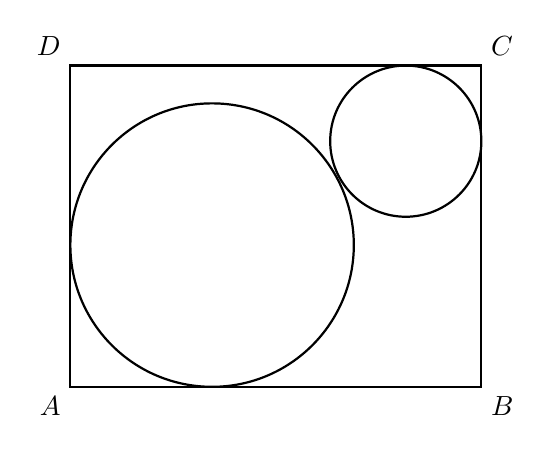
\begin{tikzpicture}[scale=0.12]

      % Titik sudut persegi panjang
      \coordinate (A) at (6.5,0);
      \coordinate (B) at (50,0);
      \coordinate (C) at (50,34);
      \coordinate (D) at (6.5,34);

      % Persegi panjang
      \draw[thick] (A)--(B)--(C)--(D)--cycle;

      % Lingkaran besar
      \draw[thick] (21.5,15) circle (15);

      % Lingkaran kecil
      \draw[thick] (42,26) circle (8);

      % Label titik
      \node[below left] at (A) {$A$};
      \node[below right] at (B) {$B$};
      \node[above right] at (C) {$C$};
      \node[above left] at (D) {$D$};

    \end{tikzpicture}
  \end{center}
  Dua lingkaran dengan jari-jari \(17\) dan \(9\) saling bersinggungan.
  Jika \(\overline{AB}=50\), maka tentukan luas persegi panjang \(ABCD\).

  \answerbox
\end{problem}

\begin{problem}
  Diberikan \(\triangle ABC\) dengan
  $
    \overline{AB}=20,\; \overline{BC}=22,\; \overline{CA}=2\sqrt{129}.
  $
  Titik \(T\) diletakkan di dalam segitiga tersebut sedemikian sehingga
  \[
    \angle TAC+\angle TBC=90^\circ-\angle ACB.
  \]
  Tentukan nilai minimum dari panjang \(CT\).

  \answerbox
\end{problem}

\begin{problem}
  Pada gambar berikut, diketahui bahwa
  $
    \overline{AE} = 25\% \text{ dari } \overline{AC}
  $
  dan
  $
    \overline{AF} = \overline{ED}.
  $
  Jika luas segitiga \(ABC\) adalah \(636\text{ cm}^2\), tentukan luas daerah yang diarsir.
  \begin{center}
    \begin{tikzpicture}[scale=0.9]

      % Titik
      \coordinate (A) at (0,5);
      \coordinate (B) at (-1,0);
      \coordinate (C) at (6,3);

      % D di BC
      \coordinate (D) at ($(B)!0.65!(C)$);

      % F di AC atas
      \coordinate (F) at ($(A)!0.55!(C)$);

      \coordinate (E) at (intersection cs:
      first line={(A)--(D)},
      second line={(F)--(B)});

      % Arsiran kiri
      \fill[gray!55] (A)--(B)--(E)--cycle;

      % Arsiran kanan
      \fill[gray!55] (F)--(C)--(D)--(E)--cycle;

      % Segitiga utama
      \draw[thick] (A)--(B)--(C)--cycle;

      % Garis dalam
      \draw[thick] (B)--(F);
      \draw[thick] (A)--(D);

      % Label
      \node[above] at (A) {$A$};
      \node[below] at (B) {$B$};
      \node[right] at (C) {$C$};
      \node[right] at (D) {$D$};
      \node[below] at (E) {$E$};
      \node[above] at (F) {$F$};

    \end{tikzpicture}
  \end{center}

  \answerbox
  % KJ : 318
\end{problem}

\newpage
\title{Solusi Tryout 2 Pembinaan OSK Matematika}
\author{MAN 1 Pasuruan}
\date{}
\maketitle
\vspace{-2cm}
\section*{Pilihan Ganda}

\begin{answer}[A. 0]
  Mari kita perhatikan pola perkalian dari beberapa suku pertama barisan tersebut:
  \begin{itemize}
    \item Untuk $n=1$: $121 = 11 \times 11$
    \item Untuk $n=2$: $11211 = 111 \times 101$
    \item Untuk $n=3$: $1112111 = 1111 \times 1001$
    \item Untuk $n=4$: $111121111 = 11111 \times 10001$
  \end{itemize}
  Berdasarkan pola untuk $n$ yang kecil tersebut, kita dapat menggeneralisasi barisan ini. Suku ke-$n$ selalu merupakan hasil kali dari dua faktor.
  Dengan demikian, bentuk umum suku ke-$n$ dari barisan tersebut adalah:
  $$ a_n = \left( \frac{10^{n+1}-1}{9} \right) (10^n+1), \quad n \ge 1. $$
  Karena setiap suku $a_n$ selalu dapat direpresentasikan sebagai perkalian dua bilangan bulat yang masing-masing lebih besar dari $1$, maka tidak ada satu pun suku dalam barisan tersebut yang merupakan bilangan prima (semuanya adalah bilangan komposit).
\end{answer}

\begin{answer}[C. $2^{607}-1$]
  Bilangan prima yang kurang dari $10$ adalah $2, 3, 5,$ dan $7$. Kita dapat semua opsi yang ada, saat menguji C ($2^{607}-1$) perhatikan bahwa:
  \begin{itemize}
    \item \textbf{Mod 2:} Merupakan bilangan ganjil, sehingga tidak habis dibagi $2$.
    \item \textbf{Mod 3:} $2^{607}-1 \equiv (-1)^{607}-1 \equiv -2 \equiv 1 \pmod 3$.
    \item \textbf{Mod 5:} Karena $2^4 \equiv 1 \pmod 5$ dan $607 = 4(151)+3$, maka $2^{607}-1 \equiv 2^3-1 \equiv 7 \equiv 2 \pmod 5$.
    \item \textbf{Mod 7:} Karena $2^3 \equiv 1 \pmod 7$ dan $607 = 3(202)+1$, maka $2^{607}-1 \equiv 2^1-1 \equiv 1 \pmod 7$.
  \end{itemize}

  Karena $2^{607}-1$ tidak habis dibagi $2, 3, 5,$ maupun $7$, maka ini adalah bilangan yang dicari.

  Sebagai pembuktian opsi lain salah:
  \begin{itemize}
    \item $2^{606}-1 \equiv (-1)^{606}-1 \equiv 0 \pmod 3$
    \item $2^{606}+1 \equiv 2^2+1 \equiv 5 \equiv 0 \pmod 5$
    \item $2^{607}+1 \equiv (-1)^{607}+1 \equiv 0 \pmod 3$
    \item $2^{607}+3^{607}$ habis dibagi $(2+3)=5$ karena pangkatnya ganjil.
  \end{itemize}
\end{answer}

\begin{answer}[B. 12]
  Diketahui persamaan $2^{a_7} = 2^{27} \cdot a_7$.
  Persamaan ini dapat ditulis ulang menjadi:
  $$ 2^{a_7 - 27} = a_7 $$
  Misalkan $k = a_7 - 27$, maka persamaan menjadi:
  $$ 2^k = k + 27 $$
  Karena $a_n$ adalah barisan bilangan bulat positif, maka $a_7 \ge 1$. Oleh karena itu, $k$ haruslah bilangan bulat. Agar $2^k$ menghasilkan bilangan bulat positif (karena $k+27 \ge 1$), maka $k \ge 0$.
  Kita uji nilai $k \ge 0$:
  \begin{itemize}
    \item Jika $k = 4$, $2^4 = 16$ dan $4 + 27 = 31$ (Tidak memenuhi).
    \item Jika $k = 5$, $2^5 = 32$ dan $5 + 27 = 32$ (Memenuhi).
  \end{itemize}
  Perhatikan bahwa $2^k>k+27$ untuk $k > 5$, sehingga solusi satu-satunya adalah $k=5$. Dengan demikian, $a_7 = k + 27 = 32$.\\
  Barisan tersebut adalah barisan aritmetika, sehingga $a_n = a_0 + nd$. Karena barisan berupa bilangan bulat positif yang naik ketat, maka $a_0 \ge 1$ dan beda $d \ge 1$ adalah bilangan bulat.
  Diketahui $a_7 = 32$:
  $$ a_0 + 7d = 32 \implies a_0 = 32 - 7d $$
  Agar $a_0 \ge 1$, maka:
  $$ 32 - 7d \ge 1 \implies 7d \le 31 \implies d \le 4 $$
  Kita ingin meminimumkan $a_2$:
  $$ a_2 = a_7 - 5d = 32 - 5d $$
  Untuk meminimumkan $a_2$, kita harus memaksimalkan $d$. Nilai bilangan bulat maksimum untuk $d$ adalah $4$.
  Jika $d = 4$, maka $a_0 = 32 - 28 = 4$ (memenuhi $a_0 \ge 1$).
  Maka nilai minimum $a_2$ adalah:
  $$ a_2 = 32 - 5(4) = \boxed{12} $$
\end{answer}

\begin{answer}[C. 3]
  Misalkan $v_p(x)$ menyatakan eksponen tertinggi dari bilangan prima $p$ yang membagi $x$. Berdasarkan sifat eksponen, berlaku $\sum v_p(x_i) = v_p(\prod x_i)$ dan $\max(v_p(x_i), v_p(x_j)) = v_p(\text{lcm}(x_i,x_j))$. Nilai FPB ditentukan oleh $\min(v_p(a), v_p(b), v_p(c), v_p(d))$.

  \begin{itemize}
    \item Untuk $p = 2$:
          Diketahui $v_2(abcd) = 6$. Karena $\max(v_2(b), v_2(c)) = 1$, maka $v_2(b), v_2(c) \le 1$.
          Karena $\max(v_2(a), v_2(b)) = 3$ dan $\max(v_2(b), v_2(d)) = 2$, mutlak diperoleh $v_2(a) = 3$ dan $v_2(d) = 2$.
          Substitusi ke jumlahan: $3 + v_2(b) + v_2(c) + 2 = 6 \implies v_2(b) + v_2(c) = 1$.
          Karena bernilai non-negatif, salah satu pasti bernilai $0$.
          Maka, $\min(v_2(a), v_2(b), v_2(c), v_2(d)) = 0$.

    \item Untuk $p = 3$:
          Diketahui $v_3(abcd) = 9$. Karena $\max(v_3(a), v_3(b)) = 2$, maka $v_3(a), v_3(b) \le 2$.
          KPK antar sisa kombinasi bernilai $3^3$, sehingga mutlak diperoleh $v_3(c) = 3$ dan $v_3(d) = 3$.
          Substitusi ke jumlahan: $v_3(a) + v_3(b) + 3 + 3 = 9 \implies v_3(a) + v_3(b) = 3$.
          Karena dibatasi maksimal $2$, distribusi nilai $\{v_3(a), v_3(b)\}$ mutlak $\{1, 2\}$.
          Maka, $\min(v_3(a), v_3(b), v_3(c), v_3(d)) = 1$.

    \item Untuk $p = 5$:
          Diketahui $v_5(abcd) = 7$. Pada himpunan $\{b, c, d\}$, nilai maksimum dari setiap pasangan adalah $2$.
          Karena $\max(v_5(a), v_5(b)) = 3$, mutlak diperoleh $v_5(a) = 3$.
          Substitusi ke jumlahan: $3 + v_5(b) + v_5(c) + v_5(d) = 7 \implies v_5(b) + v_5(c) + v_5(d) = 4$.
          Dengan batas maksimal masing-masing adalah $2$, distribusi himpunannya mutlak $\{2, 2, 0\}$.
          Maka, $\min(v_5(a), v_5(b), v_5(c), v_5(d)) = 0$.
  \end{itemize}

  Oleh karena itu, diperoleh:
  \[
    \gcd(a,b,c,d) = 2^0 \cdot 3^1 \cdot 5^0 = \boxed{3}
  \]
\end{answer}

\begin{answer}[C. 5]
  Kita mencari nilai dari $6^{66} \pmod{100}$. Berdasarkan Teorema Sisa Tiongkok, tinjau kongruensi modulo $4$ dan modulo $25$.
  \begin{itemize}
    \item \textbf{Mod 4}: $6 \equiv 2 \pmod{4}$, sehingga $6^{66} \equiv 2^{66} \equiv 0 \pmod{4}$.
    \item \textbf{Mod 25}: $6$ dan $25$ relatif prima, sehingga kita dapat menggunakan Teorema Euler. Fungsi totient Euler memberikan $\phi(25) = 20$. Karena $\gcd(6, 25) = 1$, Teorema Euler menjamin $6^{20} \equiv 1 \pmod{25}$.
          Sehingga, eksponen dapat direduksi modulo 20:
          \[
            6^{66} = 6^{3 \cdot 20 + 6} \equiv (1)^3 \cdot 6^6 \pmod{25}
          \]
          Selanjutnya, hitung $6^6 \pmod{25}$ $6^2 = 36 \equiv 11 \pmod{25}$, sehingga $6^6 = (6^2)^3 \equiv 11^3 = 1331$. Karena $1331 = 25(53) + 6$, diperoleh $6^{66} \equiv 6 \pmod{25}$.
  \end{itemize}
  \noindent Misalkan $6^{66} = 25k + 6$ untuk suatu bilangan bulat $k$. Substitusi ke syarat modulo 4 menghasilkan:
  \[
    25k + 6 \equiv 0 \pmod{4} \implies k + 2 \equiv 0 \pmod{4} \implies k \equiv 2 \pmod{4}
  \]
  Dengan mensubstitusi $k = 4m + 2$, kita peroleh:
  \[
    6^{66} = 25(4m + 2) + 6 = 100m + 56 \equiv 56 \pmod{100}
  \]
  Karena dua digit terakhir adalah $56$, digit puluhan dari bilangan tersebut adalah $\boxed{5}$.
\end{answer}

\begin{answer}[B. 54]
  Tinjau $\triangle ADC$. Berdasarkan Aturan Sinus, panjang $AC$ dapat ditentukan sebagai berikut:
  \[
    \frac{\overline{AC}}{\sin \angle ADC} = \frac{\overline{AD}}{\sin \angle ACD}
  \]
  \[
    \frac{\overline{AC}}{\sin 30^\circ} = \frac{6}{\sin 45^\circ} \implies \overline{AC} = \frac{6 \cdot \frac{1}{2}}{\frac{\sqrt{2}}{2}} = 3\sqrt{2}
  \]
  Selanjutnya, tinjau $\triangle ABC$. Berdasarkan Aturan Cosinus, nilai dari $\overline{BC}^2$ adalah:
  \[
    \overline{BC}^2 = \overline{AB}^2 + \overline{AC}^2 - 2 \cdot \overline{AB} \cdot \overline{AC} \cdot \cos \angle CAB
  \]
  \[
    \overline{BC}^2 = (6\sqrt{2})^2 + (3\sqrt{2})^2 - 2(6\sqrt{2})(3\sqrt{2}) \cos 60^\circ
  \]
  \[
    \overline{BC}^2 = 72 + 18 - 2(36)\left(\frac{1}{2}\right)
  \]
  \[
    \overline{BC}^2 = 90 - 36 = \boxed{54}
  \]
\end{answer}

\begin{answer}[E. 111]
  Diketahui $\triangle ABC$ merupakan segitiga siku-siku di $A$ dengan $\angle B = 30^\circ$ dan alas $\overline{AB} = 12\sqrt{3}$. Kita tentukan panjang sisi luar kerangka terlebih dahulu. Panjang $\overline{AC} = \overline{AB} \tan 30^\circ = 12\sqrt{3} \cdot \frac{1}{\sqrt{3}} = 12$ dan $\overline{BC} = \frac{\overline{AB}}{\cos 30^\circ} = 24$. Keliling kerangka utama tersebut adalah $\overline{AB} + \overline{BC} + \overline{AC} = 12\sqrt{3} + 36$.\\
  Selanjutnya, kita hitung total panjang besi penyangga bagian dalam yang membentuk pola zigzag tak hingga. Panjang penyangga pertama adalah $\overline{AD} = \overline{AB} \sin 30^\circ = 6\sqrt{3}$. Mengingat struktur siku-siku yang berulang, panjang penyangga berikutnya berturut-turut adalah $\overline{DE} = \overline{AD} \cos 30^\circ$, $\overline{EF} = \overline{DE} \cos 30^\circ$, dan seterusnya. Panjang penyangga dalam ini membentuk deret geometri tak hingga dengan suku pertama $u_1 = 6\sqrt{3}$ dan rasio $r = \cos 30^\circ = \frac{\sqrt{3}}{2}$. Jumlah tak hingganya adalah:
  \[
    S_{\infty} = \frac{u_1}{1 - r} = \frac{6\sqrt{3}}{1 - \frac{\sqrt{3}}{2}} = \frac{12\sqrt{3}}{2 - \sqrt{3}} = 12\sqrt{3}(2 + \sqrt{3}) = 24\sqrt{3} + 36
  \]
  Total panjang besi maksimal untuk membuat satu kerangka segitiga adalah penjumlahan keliling luar dan penyangga dalam:
  \[
    L = (12\sqrt{3} + 36) + (24\sqrt{3} + 36) = 36\sqrt{3} + 72
  \]
  Berdasarkan format $a\sqrt{b} + c$, diperoleh $a = 36$, $b = 3$, dan $c = 72$. Nilai dari $a+b+c$ adalah:
  \[
    a+b+c = 36 + 3 + 72 = \boxed{111}
  \]
\end{answer}

\begin{answer}[C. 5]
  Perhatikan gambar berikut.
  \begin{center}
    \begin{tikzpicture}[scale=0.6, line join=round, line cap=round, thick]
      \coordinate (A) at (0,6);
      \coordinate (B) at (-4,0);
      \coordinate (C) at (13,0);

      \coordinate (W) at (-2,3);
      \coordinate (V) at (6.5,3);
      \coordinate (Z) at (1.667,0);

      \coordinate (X) at (intersection of A--Z and C--W);
      \coordinate (Y) at (intersection of A--Z and B--V);

      \coordinate (M) at ($(A)!-0.4!(C)$);
      \coordinate (K) at ($(A)!-0.5!(B)$);

      \draw[dashed, blue] (B) -- (M) node[midway, left] {$\parallel AZ$};
      \draw[dashed, blue] (A) -- (M) node[midway, above, font=\bfseries] {$c$};

      \draw[dashed, orange] (C) -- (K) node[midway, above] {$\parallel AZ$};
      \draw[dashed, orange] (A) -- (K) node[midway, left, font=\bfseries] {$b$};

      % \path (A) -- (B) node[midway, below right, red, font=\bfseries] {$c$};
      % \path (A) -- (C) node[midway, below left, red, font=\bfseries] {$b$};

      \draw (A) -- (B) -- (C) -- cycle;
      \draw (A) -- (Z);
      \draw (C) -- (W);
      \draw (B) -- (V);
      \draw[dashed, red, very thick] (W) -- (Y);

      \path (A) -- (W) node[midway, sloped] {$|$};
      \path (W) -- (B) node[midway, sloped] {$|$};
      \path (A) -- (V) node[midway, sloped] {$||$};
      \path (V) -- (C) node[midway, sloped] {$||$};

      \node[above] at (A) {$A$};
      \node[below left] at (B) {$B$};
      \node[below right] at (C) {$C$};
      \node[above left] at (W) {$W$};
      \node[above right] at (V) {$V$};
      \node[below] at (Z) {$Z$};
      \node[above left, xshift=-2pt, yshift=2pt] at (X) {$X$};
      \node[below right, xshift=2pt] at (Y) {$Y$};
      \node[above right, blue] at (M) {$M$};
      \node[above left, orange] at (K) {$K$};

      \foreach \p in {A,B,C,W,V,Z,X,Y,M,K}
      \fill (\p) circle (2pt);
    \end{tikzpicture}
  \end{center}
  Tarik garis sejajar $AZ$ dari $B$ memotong perpanjangan $CA$ di $M$. Karena $AZ$ membagi $\angle A$ sama besar, sifat sudut berseberangan dan sehadap mengharuskan $\triangle ABM$ sama kaki dengan ${\overline{AM}} = \overline{AB} = c$ dan alas $\overline{BM} = 2c \cos \frac{A}{2}$.
  Pada $\triangle BVM$, karena $AY \parallel BM$, berlaku $\triangle AVY \sim \triangle MVB$. Dengan $V$ sebagai titik tengah $AC$ ($\overline{AV}=b/2$), diperoleh kesebangunan:
  \begin{align*}
    \frac{\overline{AY}}{\overline{BM}} & = \frac{\overline{AV}}{\overline{AM} + \overline{AV}} = \frac{b/2}{c + b/2} = \frac{b}{2c+b} \\
    \overline{AY}                       & = \frac{b}{2c+b} \left( 2c \cos \frac{A}{2} \right) = \frac{2bc}{2c+b} \cos \frac{A}{2}
  \end{align*}
  Dengan cara serupa tarik garis sejajar $AZ$ dari $C$ memotong perpanjangan $BA$ di $K$. Segitiga $\triangle ACK$ sama kaki dengan $\overline{AK} = \overline{AC} = b$ dan alas $\overline{CK} = 2b \cos \frac{A}{2}$.
  Pada $\triangle CKW$, karena $AX \parallel CK$, berlaku $\triangle AWX \sim \triangle KWC$. Dengan $W$ sebagai titik tengah $\overline{AB}$ ($\overline{AW}=c/2$), diperoleh:
  \begin{align*}
    \frac{\overline{AX}}{\overline{CK}} & = \frac{\overline{AW}}{\overline{AK} + \overline{AW}} = \frac{c/2}{b + c/2} = \frac{c}{2b+c} \\
    \overline{AX}                       & = \frac{c}{2b+c} \left( 2b \cos \frac{A}{2} \right) = \frac{2bc}{2b+c} \cos \frac{A}{2}
  \end{align*}
  Sehingga dapat kita tentukan panjang $\overline{XZ}$ dan $\overline{YZ}$.
  \begin{align*}
    \frac{\overline{XZ}}{\overline{YZ}} = \frac{b(b+2c)}{c(2b+c)} \implies \frac{8}{5} & = \frac{k(k+2)}{2k+1}        \implies
    5k^2 + 10k                                                    = 16k + 8                                                    \\ \implies
    5k^2 - 6k - 8                                                                      & = 0 \implies (5k+4)(k-2) = 0
  \end{align*}
  Karena nilai sisi selalu positif, maka $k = 2$, yang mengimplikasikan $b = 2c$. Substitusikan ke $b+c=30$ sehingga diperoleh $3c=30 \implies c=10$.\\
  Tinjau kembali nilai $\overline{AY}$ dengan rumus garis bagi $AZ = \frac{2bc}{b+c} \cos(A/2)$:
  \begin{align*}
    \overline{AY} = \overline{AZ} - \overline{YZ} & = \overline{AZ} \left( 1 - \frac{c}{2c+2c} \right) = \frac{3}{4} \overline{AZ}       \\
    \overline{AY}                                 & = \frac{3}{4} \left( \frac{2(2c)c}{3c} \cos \frac{A}{2} \right) = c \cos \frac{A}{2}
  \end{align*}
  Terakhir, terapkan Aturan Cosinus pada $\triangle AWY$ dengan panjang $\overline{AW} = c/2$:
  \begin{align*}
    \overline{WY}^2 & = \overline{AW}^2 + \overline{AY}^2 - 2 (\overline{AW}) (\overline{AY}) \cos \frac{A}{2}                          \\
    \overline{WY}^2 & = \frac{c^2}{4} + c^2\cos^2\frac{A}{2} - 2 \left(\frac{c}{2}\right) \left(c\cos\frac{A}{2}\right) \cos\frac{A}{2} \\
    \overline{WY}^2 & = \frac{c^2}{4} \implies \overline{WY} = \frac{c}{2} = \boxed{5}
  \end{align*}

\end{answer}

\begin{answer}[C. 210]
  Pertama ilustrasikan situasi yang diberikan dalam soal.
  \begin{center}
    \begin{tikzpicture}[scale=1, line join=round, line cap=round, thick]
      \coordinate (B) at (0,0);
      \coordinate (C) at (3,0);
      \coordinate (A) at (0, {6*sin(75)});
      \coordinate (D) at ({3+6*cos(75)}, {6*sin(75)});
      \coordinate (E) at ({3+3*cos(75)}, {3*sin(75)});
      \coordinate (H) at (3, {6*sin(75)});
      \coordinate (M) at (0, {3*sin(75)});

      \draw (A) -- (B) -- (C) -- (D) -- cycle;
      \draw (A) -- (E);
      \draw[dashed, gray] (C) -- (H);
      \draw[dashed, blue] (M) -- (E);

      \path (C) -- (E) node[midway, sloped] {$|$};
      \path (E) -- (D) node[midway, sloped] {$|$};
      \path (B) -- (C) node[midway, sloped] {$|$};
      \path (A) -- (M) node[midway, sloped] {$||$};
      \path (M) -- (B) node[midway, sloped] {$||$};

      \draw (0,0.3) -- (0.3,0.3) -- (0.3,0);
      \draw (0, {6*sin(75)-0.3}) -- (0.3, {6*sin(75)-0.3}) -- (0.3, {6*sin(75)});

      \draw (D) ++(180:0.8) arc (180:255:0.8);
      \node at ($(D) + (217.5:0.5)$) {\tiny$75^\circ$};

      \node[above left] at (A) {$A$};
      \node[below left] at (B) {$B$};
      \node[below right] at (C) {$C$};
      \node[above right] at (D) {$D$};
      \node[right, xshift=2pt] at (E) {$E$};
      \node[above] at (H) {$H$};
      \node[left,blue] at (M) {$M$};

      \foreach \p in {A,B,C,D,E,H}
      \fill (\p) circle (2pt);
    \end{tikzpicture}
  \end{center}
  Misalkan $\overline{BC} = x$, maka dari $\overline{DE} = \overline{EC} = \overline{BC}$ diperoleh $\overline{CD} = 2x$. Tarik garis tinggi $CH \perp AD$, sehingga $ABCH$ membentuk persegi panjang dengan $\overline{AH} = \overline{BC} = x$ dan $\overline{AB} = CH$.
  Tinjau $\triangle CHD$ siku-siku di $H$ dengan $\angle HDC = 75^\circ$:
  $$ \begin{aligned} CH &= CD \sin 75^\circ = 2x \sin 75^\circ \\ HD &= CD \cos 75^\circ = 2x \cos 75^\circ \end{aligned} $$
  Akibatnya, panjang sisi siku-siku trapesium adalah $\overline{AB} = 2x \sin 75^\circ$ dan sisi atas $\overline{AD} = \overline{AH} + \overline{HD} = x + 2x \cos 75^\circ$\\
  Selanjutnya misalkan titik $M$ adalah titik tengah $\overline{AB}$. Tarik garis $ME$. Karena $M$ dan $E$ masing-masing adalah titik tengah dari kaki trapesium $\overline{AB}$ dan $\overline{CD}$, ruas garis $ME$ merupakan garis tengah trapesium yang sejajar dengan $\overline{AD}$ maupun $\overline{BC}$, serta tegak lurus terhadap $\overline{AB}$.
  Tentukan panjang $\overline{AM}$ dan $\overline{ME}$:
  $$ \begin{aligned} \overline{AM} &= \frac{1}{2} \overline{AB} = x \sin 75^\circ \\ \overline{ME} &= \frac{\overline{AD} + \overline{BC}}{2} = \frac{(x + 2x \cos 75^\circ) + x}{2} = x + x \cos 75^\circ \end{aligned} $$
  Tinjau $\triangle AME$ yang siku-siku di $M$. Karena titik $M$ terletak pada garis $\overline{AB}$, sudut $\angle BAE$ identik dengan $\angle MAE$. Nilai tangennya adalah:
  $$ \tan \angle BAE = \frac{\overline{ME}}{\overline{AM}} = \frac{x + x \cos 75^\circ}{x \sin 75^\circ} = \frac{1 + \cos 75^\circ}{\sin 75^\circ} $$
  Terapkan identitas sudut pertengahan $\frac{1+\cos\theta}{\sin\theta} = \cot\frac{\theta}{2}$:
  $$ \tan \angle BAE = \cot \left(\frac{75^\circ}{2}\right) = \tan (90^\circ - 37,5^\circ) = \tan 52,5^\circ $$
  Maka diperoleh $\angle BAE = 52,5^\circ = \left(\frac{105}{2}\right)^\circ$. Parameter pecahannya adalah $a=105$ dan $b=2$, yang sudah memenuhi syarat saling prima.
  Hasil akhirnya adalah $ab = 105 \times 2 = \boxed{210}$.
\end{answer}

\begin{answer}[B. 8]
  Tinjau gambar berikut
  \begin{center}
    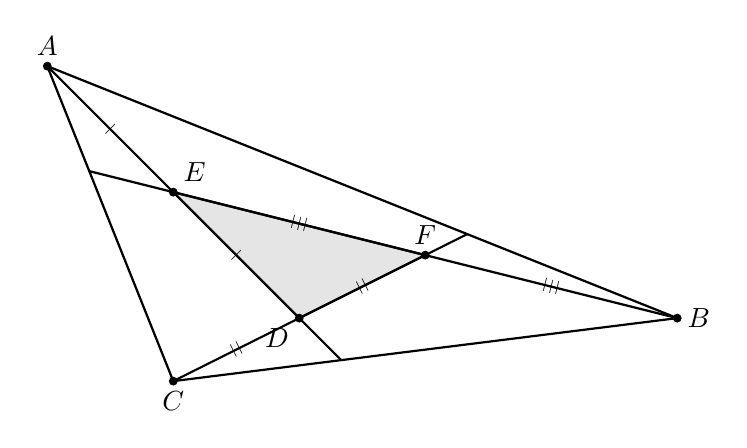
\begin{tikzpicture}[scale=0.8, line join=round, line cap=round, thick]
      \coordinate (A) at (0,5);
      \coordinate (B) at (10,1);
      \coordinate (C) at (2,0);
      \coordinate (D) at (4,1);
      \coordinate (E) at (2,3);
      \coordinate (F) at (6,2);
      \coordinate (J) at (14/3, 1/3);
      \coordinate (H) at (2/3, 10/3);
      \coordinate (I) at (20/3, 7/3);

      \fill[gray!20] (D) -- (E) -- (F) -- cycle;

      \draw (A) -- (B) -- (C) -- cycle;
      \draw (A) -- (J);
      \draw (B) -- (H);
      \draw (C) -- (I);
      \draw (D) -- (E) -- (F) -- cycle;

      \path (A) -- (E) node[midway, sloped] {\tiny$|$};
      \path (E) -- (D) node[midway, sloped] {\tiny$|$};
      \path (C) -- (D) node[midway, sloped] {\tiny$||$};
      \path (D) -- (F) node[midway, sloped] {\tiny$||$};
      \path (B) -- (F) node[midway, sloped] {\tiny$|||$};
      \path (F) -- (E) node[midway, sloped] {\tiny$|||$};

      \node[above] at (A) {$A$};
      \node[right] at (B) {$B$};
      \node[below] at (C) {$C$};
      \node[below left] at (D) {$D$};
      \node[above right] at (E) {$E$};
      \node[above] at (F) {$F$};

      \foreach \p in {A,B,C,D,E,F}
      \fill (\p) circle (2pt);
    \end{tikzpicture}
  \end{center}
  Gunakan pendekatan vektor posisi untuk menyederhanakan rumitnya perpotongan garis cevian. Misalkan vektor posisi setiap titik dinyatakan dengan notasi $\vec{v}$.
  Berdasarkan informasi pembagian ruas garis yang sama panjang di soal:
  $$ \begin{aligned} \overline{AE} &= \overline{ED} \implies \vec{E} = \frac{\vec{A} + \vec{D}}{2} \implies \vec{A} = 2\vec{E} - \vec{D} \\ \overline{CD} &= \overline{FD} \implies \vec{D} = \frac{\vec{C} + \vec{F}}{2} \implies \vec{C} = 2\vec{D} - \vec{F} \\ \overline{BF} &= \overline{FE} \implies \vec{F} = \frac{\vec{B} + \vec{E}}{2} \implies \vec{B} = 2\vec{F} - \vec{E} \end{aligned} $$
  Susun ketiga relasi tersebut ke dalam bentuk transformasi matriks linear yang memetakan titik-titik $\triangle DEF$ ke titik-titik $\triangle ABC$:
  $$ \begin{pmatrix} \vec{A} \\ \vec{B} \\ \vec{C} \end{pmatrix} = \begin{pmatrix} -1 & 2 & 0 \\ 0 & -1 & 2 \\ 2 & 0 & -1 \end{pmatrix} \begin{pmatrix} \vec{D} \\ \vec{E} \\ \vec{F} \end{pmatrix} $$
  Rasio luas kedua segitiga tersebut setara dengan nilai determinan mutlak dari matriks transformasinya. Hitung determinan matriks $3 \times 3$ ($M$) tersebut:
  $$ \begin{aligned} \det(M) &= -1(1 - 0) - 2(0 - 4) + 0 = -1 + 8 = 7 \end{aligned} $$
  Nilai determinan ini secara analitis membuktikan bahwa $[\triangle ABC] = 7 [\triangle DEF]$.
  Dengan demikian, perbandingan luas $\triangle EFD$ terhadap luas $\triangle ABC$ adalah $\frac{1}{7}$.
  Didapat $a=1$ dan $b=7$ yang terjamin saling prima.
  Nilai akhirnya adalah $a+b = 1+7 = \boxed{8}$.
\end{answer}


\section*{Isian Singkat}
\begin{answer}[278]
  Syarat habis dibagi $22$ mengimplikasikan bilangan tersebut harus genap dan merupakan kelipatan $11$.
  Jumlah total dari seluruh digit adalah $S = 1+2+3+4+5+6+7+8 = 36$. Agar kelipatan $11$, selisih antara jumlah digit di posisi ganjil ($S_{ganjil}$) dan genap ($S_{genap}$) haruslah kelipatan $11$. Karena $S_{ganjil} + S_{genap} = 36$, satu-satunya selisih yang mungkin untuk menghasilkan bilangan bulat adalah $0$.
  $$ S_{ganjil} - S_{genap} = 0 \implies S_{ganjil} = S_{genap} = 18 $$
  Kita perlu mempartisi himpunan $\{1, 2, 3, 4, 5, 6, 7, 8\}$ menjadi dua himpunan bagian beranggotakan $4$ digit yang jumlahnya masing-masing $18$. Terdapat persis $4$ pasang himpunan yang memenuhi:
  \begin{enumerate}
    \item $\{1, 2, 7, 8\}$ dan $\{3, 4, 5, 6\}$
    \item $\{1, 3, 6, 8\}$ dan $\{2, 4, 5, 7\}$
    \item $\{1, 4, 5, 8\}$ dan $\{2, 3, 6, 7\}$
    \item $\{1, 4, 6, 7\}$ dan $\{2, 3, 5, 8\}$
  \end{enumerate}
  Setiap pasang himpunan dapat ditugaskan sebagai posisi genap atau ganjil. Misalkan himpunan $E$ memuat digit untuk posisi genap dan memuat angka genap sebanyak $c(E)$. Digit terakhir mutlak menempati posisi genap, sehingga wajib dipilih dari angka genap yang tersedia di $E$. Banyaknya cara menyusun bilangan untuk suatu himpunan $E$ adalah:
  $$ (4!) \times \left( c(E) \cdot 3! \right) = 24 \times 6 \cdot c(E) = 144 \cdot c(E) $$
  Karena di setiap pasang himpunan total angka genapnya selalu terdistribusi sebanyak $4$ buah ($c(A) + c(B) = 4$), banyaknya susunan untuk satu pasang adalah:
  $$ 144 \cdot c(A) + 144 \cdot c(B) = 144 (c(A) + c(B)) = 144 \times 4 = 576 $$
  Karena ada $4$ pasang himpunan yang ekuivalen, total bilangan $N$ adalah:
  $$ N = 4 \times 576 = 2304 $$
  Selisih antara $N$ dan $2026$ adalah:
  $$ |2304 - 2026| = \boxed{278} $$
\end{answer}


\begin{answer}[699]
  Misalkan bilangan empat digit tersebut adalah $N = 1000a + 100b + 10c + d$. Gunakan sifat sisa pembagian modulo $7$:
  $$ 1000 \equiv -1 \pmod 7, \quad 100 \equiv 2 \pmod 7, \quad 10 \equiv 3 \pmod 7, \quad 1 \equiv 1 \pmod 7 $$
  Sehingga nilai $N$ modulo $7$ dapat diekspresikan sebagai:
  $$ N \equiv -a + 2b + 3c + d \pmod 7 $$
  Misalkan $N \equiv k \pmod 7$. Saat satu digit diubah menjadi angka $1$, bilangan tersebut habis dibagi $7$. Berdasarkan nilai tempatnya, hal ini menghasilkan empat relasi:
  \begin{align*}
    N - 1000a + 1000(1) \equiv 0 \pmod 7 & \implies k + a - 1 \equiv 0 \implies a \equiv 1-k \pmod 7   \\
    N - 100b + 100(1) \equiv 0 \pmod 7   & \implies k - 2b + 2 \equiv 0 \implies 2b \equiv k+2 \pmod 7 \\
    N - 10c + 10(1) \equiv 0 \pmod 7     & \implies k - 3c + 3 \equiv 0 \implies 3c \equiv k+3 \pmod 7 \\
    N - d + 1(1) \equiv 0 \pmod 7        & \implies k - d + 1 \equiv 0 \implies d \equiv k+1 \pmod 7
  \end{align*}
  Substitusikan keempat relasi tersebut ke persamaan modulus awal $N$:
  \begin{align*}
    k  & \equiv -(1-k) + (k+2) + (k+3) + (k+1) \pmod 7          \\
    k  & \equiv 4k + 5 \pmod 7                                  \\
    3k & \equiv -5 \equiv 2 \pmod 7 \implies k \equiv 3 \pmod 7
  \end{align*}
  Dengan $k=3$, tentukan rentang digit penyusun bilangan:
  \begin{align*}
    a  & \equiv 1-3 \equiv 5 \pmod 7 \implies a = 5                              \\
    2b & \equiv 3+2 \equiv 5 \implies b \equiv 6 \pmod 7 \implies b = 6          \\
    3c & \equiv 3+3 \equiv 6 \implies c \equiv 2 \pmod 7 \implies c \in \{2, 9\} \\
    d  & \equiv 3+1 \equiv 4 \pmod 7 \implies d = 4
  \end{align*}
  Agar $N$ bernilai maksimum, pilih digit opsional terbesar yaitu $c = 9$. Maka, diperoleh susunan digit maksimal $N = 5694$.
  Berdasarkan format pembagian bersisa $N = 1000Q + R$:
  \begin{align*}
    Q & = \lfloor 5694 / 1000 \rfloor = 5 \\
    R & = 5694 \pmod{1000} = 694
  \end{align*}
  Nilai akhir dari $Q+R$ adalah:
  $$ Q+R = 5 + 694 = \boxed{699} $$
\end{answer}

\begin{answer}[2]
  Nilai fungsi totient Euler $\phi(m)$ selalu mengembalikan bilangan genap untuk setiap bilangan asli $m \ge 3$. Mengingat satu-satunya bilangan prima genap adalah $2$, syarat $\phi(m)$ bernilai prima mutlak mengharuskan $\phi(m) = 2$ untuk rentang $m \ge 3$.
  Untuk nilai $m < 3$, diketahui $\phi(1) = 1$ dan $\phi(2) = 1$, yang keduanya bukan bilangan prima.

  Kita tentukan semua nilai $m$ yang memenuhi $\phi(m) = 2$. Berdasarkan definisi fungsi totient, nilai $m$ yang valid hanyalah himpunan $\{3, 4, 6\}$.
  Soal meminta barisan bilangan bulat berurutan $n, n+1, \dots, n+k-1$ terpanjang yang seluruh elemen fungsinya bernilai prima. Ini ekuivalen dengan mencari sub-barisan berurutan terpanjang dari himpunan $\{3, 4, 6\}$.

  Pasangan bilangan berurutan yang dapat dibentuk murni hanyalah $3$ dan $4$.
  Karena tidak ada lagi bilangan yang berurutan setelahnya (angka $5$ putus karena $\phi(5)=4$), panjang barisan maksimum adalah $2$.
  Nilai asli terbesar $k$ yang memenuhi adalah $\boxed{2}$.
\end{answer}

\begin{answer}[8]
  Tinjau paritas dari $n$ untuk menentukan faktor prima terkecil $p_n$ dari $n^8+1$.
  \begin{itemize}
    \item  Jika $n$ ganjil, $n^8+1$ mutlak bernilai genap. Faktor prima terkecil dari bilangan genap selalu $p_n = 2$. Pada rentang $1 \le n \le 2021$, terdapat persis $1011$ bilangan ganjil.
    \item Jika $n$ genap, $n^8+1$ bernilai ganjil. Misalkan $p$ adalah salah satu faktor primanya, maka berlaku kongruensi:
          \begin{align*}
            n^8 + 1 & \equiv 0 \pmod p                                   \implies
            n^8     \equiv -1 \pmod p \implies n^{16} \equiv 1 \pmod p
          \end{align*}
          Berdasarkan sifat orde perkalian, orde dari $n$ modulo $p$ mutlak membagi $16$ tetapi tidak membagi $8$, sehingga ordenya tepat bernilai $16$.
          Teorema Kecil Fermat menjamin orde tersebut membagi $p-1$. Maka diperoleh $16 \mid (p-1)$, yang secara langsung mengimplikasikan $p \equiv 1 \pmod{16}$.
          Oleh karena itu, faktor prima terkecil $p_n$ mutlak memenuhi kongruensi $p_n \equiv 1 \pmod{16}$ untuk setiap $n$ genap. Pada rentang yang sama, terdapat $1010$ bilangan genap.
  \end{itemize}
  Terkahir hitung sisa pembagian deret jumlahan $\sum p_n$ modulo $16$:
  \begin{align*}
    \sum_{n=1}^{2021} p_n & \equiv 1011(2) + 1010(1) \pmod{16}                             \\
    \sum_{n=1}^{2021} p_n & \equiv (16 \times 63 + 3)(2) + (16 \times 63 + 2)(1) \pmod{16} \\
    \sum_{n=1}^{2021} p_n & \equiv 3(2) + 2(1) \equiv 6 + 2 \equiv \boxed{8} \pmod{16}
  \end{align*}
\end{answer}

\begin{answer}[4]
  Tinjau banyaknya angka nol berurutan di akhir $20!$ dengan menghitung total eksponen faktor prima $5$ menggunakan rumus Legendre diperoleh
  $ \lfloor 20/5 \rfloor = 4 $.
  Karena nilai $20!$ diakhiri oleh tepat $4$ buah angka nol berurutan, susunan digit pada ujung format $\dots bc000$ mengharuskan $c = 0$.
  Dengan menyubstitusikan $c=0$, format angka menjadi $24329a20081766b0000$.\\
  Gunakan sifat keterbagian bilangan untuk membedah digit $a$ dan $b$.
  Sifat kelipatan $9$ menjamin jumlah seluruh digit habis dibagi $9$:
  \begin{align*}
    2+4+3+2+9+a+2+0+0+8+1+7+6+6+b+0+0+0+0 & \equiv 0 \pmod 9 \\
    50 + a + b                            & \equiv 0 \pmod 9 \\
    a + b                                 & \equiv 4 \pmod 9
  \end{align*}
  Sifat kelipatan $11$ menjamin selisih jumlah digit posisi ganjil dan genap (dihitung dari kiri ke kanan) habis dibagi $11$:
  \begin{align*}
    S_{ganjil}             & = 2+3+9+2+0+1+6+b+0+0 = 23+b                         \\
    S_{genap}              & = 4+2+a+0+8+7+6+0+0 = 27+a                           \\
    S_{ganjil} - S_{genap} & \equiv 0 \pmod{11}                                   \\
    (23+b) - (27+a)        & \equiv 0 \pmod{11} \implies b - a \equiv 4 \pmod{11}
  \end{align*}
  Berdasarkan batasan nilai digit $0 \le a,b \le 9$, rentang $b-a$ yang memenuhi kongruensi hanyalah $4$ atau $-7$. Sementara untuk persamaan pertama, rentang $|a+b|$ berada pada himpunan $\{4, 13\}$.
  Eksekusi kombinasi sistem persamaan linearnya:
  \begin{itemize}
    \item Kondisi 1: $b - a = 4$
          \begin{itemize}
            \item Jika $a + b = 4 \implies 2b = 8 \implies b = 4, a = 0$ (Memenuhi digit)
            \item Jika $a + b = 13 \implies 2b = 17$ (Tidak bulat)
          \end{itemize}
    \item Kondisi 2: $b - a = -7$
          \begin{itemize}
            \item Jika $a + b = 4 \implies 2b = -3$ (Tidak bulat)
            \item Jika $a + b = 13 \implies 2b = 6 \implies b = 3, a = 10$ (Bukan digit)
          \end{itemize}
  \end{itemize}
  Satu-satunya solusi adalah $a=0, b=4$, dan $c=0$.
  Hasil jumlahan akhirnya adalah
  $$ a+b+c = 0+4+0 = \boxed{4} $$
\end{answer}

\begin{answer}[303]
  Pertama ilustrasikan situasi yang diberikan dalam soal.
  \begin{center}
    \begin{tikzpicture}[scale=0.35, line join=round, line cap=round, thick, font=\footnotesize, every node/.style={font=\scriptsize}]
      \coordinate (O) at (0,0);
      \coordinate (A) at (0,10);
      \coordinate (B) at ({10*cos(-30)}, {10*sin(-30)});
      \coordinate (C) at (-10,0);
      \coordinate (M) at ($(A)!0.5!(B)$);
      \coordinate (N) at ($(A)!0.5!(C)$);

      \draw (O) circle (10);
      \draw (A) -- (B) -- (C) -- cycle;

      \draw[dashed, blue] (O) -- (A) node[midway, right] {$10$};
      \draw[dashed, blue] (O) -- (M) node[midway, below right] {$5$};
      \draw[dashed, blue] (O) -- (N) node[midway, below left] {$5\sqrt{2}$};

      % Sudut siku-siku pake pic
      \pic[draw, red, angle radius=3mm] {right angle=A--M--O};
      \pic[draw, red, angle radius=3mm] {right angle=O--N--A};

      % Sudut kemiringan pake pic
      \pic[draw, red, angle radius=1cm, "\tiny$30^\circ$", angle eccentricity=0.7] {angle=O--A--B};
      \pic[draw, red, angle radius=0.9cm, "\tiny$45^\circ$", angle eccentricity=0.6] {angle=C--A--O};

      \fill (O) circle (4pt) node[below] {$O$};
      \fill (A) circle (4pt) node[above] {$A$};
      \fill (B) circle (4pt) node[below right] {$B$};
      \fill (C) circle (4pt) node[left] {$C$};
      \fill (M) circle (4pt) node[right] {$M$};
      \fill (N) circle (4pt) node[above left] {$N$};
    \end{tikzpicture}
  \end{center}
  Misalkan $M$ dan $N$ berturut-turut adalah titik tengah tali busur $AB$ dan $AC$. Garis dari pusat $O$ ke titik tengah tali busur mutlak tegak lurus terhadap tali busur tersebut ($OM \perp AB$ dan $ON \perp AC$).
  Tinjau $\triangle OMA$ yang siku-siku di $M$:
  \begin{align*}
    AM              & = \sqrt{OA^2 - OM^2} = \sqrt{10^2 - 5^2} = \sqrt{75} = 5\sqrt{3} \implies AB = 10\sqrt{3}  \\
    \cos \angle OAM & = \frac{AM}{OA} = \frac{5\sqrt{3}}{10} = \frac{\sqrt{3}}{2} \implies \angle OAM = 30^\circ
  \end{align*}
  Tinjau $\triangle ONA$ yang siku-siku di $N$:
  \begin{align*}
    AN              & = \sqrt{OA^2 - ON^2} = \sqrt{10^2 - (5\sqrt{2})^2} = \sqrt{50} = 5\sqrt{2} \implies AC = 10\sqrt{2} \\
    \cos \angle OAN & = \frac{AN}{OA} = \frac{5\sqrt{2}}{10} = \frac{\sqrt{2}}{2} \implies \angle OAN = 45^\circ
  \end{align*}
  Pusat lingkaran $O$ diasumsikan berada di dalam $\triangle ABC$ untuk mendapatkan panjang maksimal $BC$ yang menghasilkan format akar tak nol. Sudut puncaknya adalah:
  $$ \angle BAC = \angle OAM + \angle OAN = 30^\circ + 45^\circ = 75^\circ $$
  Gunakan Aturan Cosinus pada $\triangle ABC$ dengan $\cos 75^\circ = \cos(45^\circ+30^\circ) = \frac{\sqrt{6}-\sqrt{2}}{4}$:
  \begin{align*}
    BC^2 & = AB^2 + AC^2 - 2(AB)(AC) \cos 75^\circ                                                       \\
    BC^2 & = (10\sqrt{3})^2 + (10\sqrt{2})^2 - 2(100\sqrt{6}) \left( \frac{\sqrt{6}-\sqrt{2}}{4} \right) \\
    BC^2 & = 300 + 200 - 50\sqrt{6} (\sqrt{6}-\sqrt{2})                                                  \\
    BC^2 & = 500 - 300 + 50\sqrt{12}                                                                     \\
    BC^2 & = 200 + 100\sqrt{3}
  \end{align*}
  Diperoleh $a = 200$, $b = 100$, dan $c = 3$. Nilai dari $a+b+c$ adalah:
  $$ a+b+c = 200 + 100 + 3 = \boxed{303} $$
\end{answer}

\begin{answer}[10]
  Pertama-tama ilustrasikan terlebih dahulu
  \begin{center}
    \begin{tikzpicture}[scale=0.8, line join=round, line cap=round, thick]
      \coordinate (B) at (0,0);
      \coordinate (C) at (10,0);
      \coordinate (A) at (4,6);

      \coordinate (E) at ($(A)!0.5!(C)$);
      \coordinate (F) at ($(A)!0.5!(B)$);

      \coordinate (G) at (intersection of B--E and C--F);
      \coordinate (Y) at ($(B)!0.5!(E)$);
      \coordinate (Z) at ($(C)!0.5!(F)$);

      \fill[orange!30] (G) -- (Y) -- (Z) -- cycle;

      \draw (A) -- (B) -- (C) -- cycle;
      \draw (B) -- (E);
      \draw (C) -- (F);
      \draw[red, very thick] (Y) -- (Z);

      \path (A) -- (E) node[midway, sloped] {$|$};
      \path (E) -- (C) node[midway, sloped] {$|$};
      \path (A) -- (F) node[midway, sloped] {$||$};
      \path (F) -- (B) node[midway, sloped] {$||$};

      \node[above] at (A) {$A$};
      \node[below left] at (B) {$B$};
      \node[below right] at (C) {$C$};
      \node[above right] at (E) {$E$};
      \node[above left] at (F) {$F$};
      \node[above, yshift=2pt] at (G) {\small $G$};
      \node[left] at (Y) {\small $Y$};
      \node[right] at (Z) {\small $Z$};

      \path (B) -- (Y) node[midway, below, font=\small] {$2x$};
      \path (Y) -- (G) node[midway,above left, font=\scriptsize] {$x$};
      \path (G) -- (E) node[midway, above, font=\small] {$2x$};

      \path (C) -- (Z) node[midway, below, font=\small] {$2y$};
      \path (Z) -- (G) node[midway,above right, font=\scriptsize] {$y$};
      \path (G) -- (F) node[midway, above, font=\small] {$2y$};

      \foreach \p in {A,B,C,E,F,G,Y,Z}
      \fill (\p) circle (2pt);
    \end{tikzpicture}
  \end{center}
  Titik berat $G$ membagi setiap garis berat dengan rasio $2:1$. Misalkan panjang $BE = 6x$, maka:
  $$ BG = \frac{2}{3}(6x) = 4x \quad \text{dan} \quad GE = \frac{1}{3}(6x) = 2x $$
  Diketahui $Y$ adalah titik tengah garis berat $BE$, sehingga jarak dari sudut $B$ adalah:
  $$ BY = \frac{1}{2}(6x) = 3x $$
  Karena $BY < BG$, posisi $Y$ pasti berada di antara $B$ dan $G$. Panjang segmen $YG$ adalah:
  $$ YG = BG - BY = 4x - 3x = x $$
  Hal ini menunjukkan rasio $YG$ terhadap $BG$ adalah $\frac{x}{4x} = \frac{1}{4}$.
  Dengan penganalogian yang sama pada garis berat $CF = 6y$, titik tengah $Z$ membagi ruas $CG$ dengan rasio $\frac{ZG}{CG} = \frac{y}{4y} = \frac{1}{4}$.\\
  Tinjau $\triangle GYZ$ dan $\triangle GBC$. Karena titik $Y$ dan $Z$ masing-masing terletak pada segmen pembentuk $\angle BGC$, kedua segitiga berbagi sudut puncak yang persis sama di $G$. Perbandingan luasnya adalah hasil kali perbandingan sisi apitnya:
  $$ \frac{[\triangle GYZ]}{[\triangle GBC]} = \frac{YG}{BG} \times \frac{ZG}{CG} = \frac{1}{4} \times \frac{1}{4} = \frac{1}{16} $$
  Berdasarkan sifat titik berat, luas segitiga yang dibentuk oleh alas dan titik berat selalu sepertiga dari luas total:
  $$ [\triangle GBC] = \frac{1}{3} [\triangle ABC] = \frac{1}{3} (480) = 160 $$
  Sehingga luas $\triangle GYZ$ adalah
  $$ [\triangle GYZ] = \frac{1}{16} [\triangle GBC] = \frac{1}{16} (160) = \boxed{10} $$
\end{answer}

\begin{answer}[1800]
  Perhatikan gambar berikut
  \begin{center}
    \begin{tikzpicture}[scale=0.15, line join=round, line cap=round, thick]
      \coordinate (A) at (0,0);
      \coordinate (B) at (50,0);
      \coordinate (C) at (50,36);
      \coordinate (D) at (0,36);

      \coordinate (O1) at (17,17);
      \coordinate (O2) at (41,27);
      \coordinate (P) at (41,17);

      \draw (A) -- (B) node[midway, below] {$50$} -- (C) node[midway, right] {$h$} -- (D) -- cycle;
      \draw (O1) circle (17);
      \draw (O2) circle (9);

      \draw[dashed, blue] (O1) -- (O2) node[midway, above left] {$26$};
      \draw[dashed, blue] (O1) -- (17,0) node[midway, left] {$17$};
      \draw[dashed, blue] (O2) -- (41,36) node[midway, right] {$9$};
      \draw[dashed, orange] (O1) -- (P) node[midway, below] {$24$};
      \draw[dashed, orange] (O2) -- (P) node[midway, right] {\scriptsize $h-26$};

      \pic[draw, angle radius=3mm] {right angle=O2--P--O1};

      \fill (O1) circle (6pt) node[left] {$O_1$};
      \fill (O2) circle (6pt) node[right] {$O_2$};
      \fill (P) circle (6pt) node[below left] {$P$};
      \node[below left] at (A) {$A$};
      \node[below right] at (B) {$B$};
      \node[above right] at (C) {$C$};
      \node[above left] at (D) {$D$};
    \end{tikzpicture}
  \end{center}
  Misalkan $O_1$ adalah pusat lingkaran besar dengan jari-jari $R=17$, dan $O_2$ adalah pusat lingkaran kecil dengan jari-jari $r=9$.
  Tarik garis horizontal dari $O_1$ ke kanan dan garis vertikal dari $O_2$ ke bawah hingga berpotongan di titik $P$, membentuk $\triangle O_1PO_2$ yang siku-siku di $P$.
  Jarak antara kedua pusat lingkaran ($O_1O_2$) adalah
  $$ \overline{O_1O_2} = R + r = 17 + 9 = 26 $$
  Selnjutnya untuk panjang alas segitiga ($O_1P$) diperoleh
  $$ \overline{O_1P} = AB - R - r = 50 - 17 - 9 = 24 $$
  Misalkan tinggi persegi panjang adalah $h$, maka
  $$ \overline{PO_2} = h - R - r = h - 17 - 9 = h - 26 $$
  Menggunakan Teorema Pythagoras pada $\triangle O_1PO_2$:
  \begin{align*}
    O_1P^2 + PO_2^2   & = O_1O_2^2 \\
    24^2 + (h - 26)^2 & = 26^2     \\
    576 + (h - 26)^2  & = 676      \\
    (h - 26)^2        & = 100
  \end{align*}
  Karena jarak bernilai positif, maka diambil $h - 26 = 10 \implies h = 36$.
  Sehingga luas persegi panjang $ABCD$
  $$ [ABCD] = AB \times h = 50 \times 36 = \boxed{1800} $$
\end{answer}

\begin{answer}[10]
  Misalkan $\angle ACB = \gamma$. Diketahui persamaan sudut $\angle TAC + \angle TBC = 90^\circ - \gamma$.
  Pada $\triangle ABC$, berlaku sifat jumlahan sudut $\angle A + \angle B + \gamma = 180^\circ$.
  Substitusikan jumlahan ini dengan memecah sudut yang diketahui:
  $$ \begin{aligned} \angle TAC + \angle TBC &= (\angle A - \angle TAB) + (\angle B - \angle TBA) \\ &= (\angle A + \angle B) - (\angle TAB + \angle TBA) \\ &= (180^\circ - \gamma) - (180^\circ - \angle ATB) \\ &= \angle ATB - \gamma \end{aligned} $$
  Sehingga, diperoleh hubungan sudut yang sangat penting
  $$ \angle ATB - \gamma = 90^\circ - \gamma \implies \angle ATB = 90^\circ $$
  \begin{center}
    \begin{tikzpicture}[scale=0.25, line join=round, line cap=round, thick]
      \coordinate (M) at (0,0);
      \coordinate (B) at (10,0);
      \coordinate (A) at (-10,0);

      \draw[dashed, gray] (M) circle (10);

      \coordinate (C) at ({20*cos(70)}, {20*sin(70)});
      \coordinate (T) at ({10*cos(70)}, {10*sin(70)});

      \draw (A) -- (M) node[midway, below] {\small$10$} -- (B) node[midway, below] {\small$10$} -- (C) node[midway, right, xshift=2pt] {\small$22$} -- cycle;
      \path (A) -- (C) node[midway, left] {\small$2\sqrt{129}$};
      \draw[dashed, blue] (M) -- (C);
      \draw[orange] (A) -- (T) -- (B);

      \pic[draw, angle radius=3mm] {right angle=A--T--B};

      \fill (A) circle (5pt) node[left] {$A$};
      \fill (B) circle (5pt) node[right] {$B$};
      \fill (C) circle (5pt) node[above] {$C$};
      \fill (M) circle (5pt) node[below] {$M$};
      \fill (T) circle (5pt) node[above left] {$T$};
    \end{tikzpicture}
  \end{center}
  Sudut siku-siku ini secara geometri memastikan bahwa titik $T$ mutlak berada pada keliling setengah lingkaran dengan diameter sisi $AB$.
  Misalkan titik $M$ adalah titik tengah $AB$, maka $M$ berkedudukan sebagai pusat lingkaran luar tersebut dengan jari-jari $R = \frac{1}{2}\overline{AB} = 10$. Akibatnya, $\overline{MT} = 10$.\\
  Untuk meminimumkan panjang segmen $CT$, titik $T$ wajib diposisikan segaris pada ruas garis yang menghubungkan titik $C$ langsung ke titik pusat $M$.
  Dengan demikian panjang garis berat $CM$ dapat dihitung melalui Teorema Apollonius pada $\triangle ABC$:
  $$ \begin{aligned} \overline{AC}^2 + \overline{BC}^2 &= 2(\overline{CM}^2 + \overline{AM}^2) \\ (2\sqrt{129})^2 + 22^2 &= 2(\overline{CM}^2 + 10^2) \\ 516 + 484 &= 2(\overline{CM}^2 + 100) \\ 1000 &= 2\overline{CM}^2 + 200 \\ 2\overline{CM}^2 &= 800 \implies \overline{CM}^2 = 400 \implies \overline{CM} = 20 \end{aligned} $$
  Karena $T$ memotong ruas $CM$ dalam jarak terdekat ke $C$, nilai minimum dari $\overline{CT}$ adalah:
  $$ \overline{CT}_{min} = \overline{CM} - \overline{MT} = 20 - 10 = \boxed{10} $$
\end{answer}


\begin{answer}[318]
  Diketahui $\overline{AE} = \frac{1}{4}\overline{AC}$, $\overline{AF} = \overline{ED}$ dan $[\triangle ABC] =  636$. Misalkan luas daerah yang diarsir adalah $S$.\\
  Pertama tarik garis tinggi $h_E$ dari titik $E$ tegak lurus ke $AC$, dan $h_C$ dari titik $C$ tegak lurus ke perpanjangan $AD$.
  Tinjau $\triangle ACE$. Luasnya dapat dihitung melalui dua perspektif alas dan tinggi yang berbeda:
  \begin{itemize}
    \item Alas $AC$ dengan tinggi $h_E \implies [\triangle ACE] = \frac{1}{2} AC \cdot h_E$
    \item Alas $AE$ dengan tinggi $h_C \implies [\triangle ACE] = \frac{1}{2} AE \cdot h_C$
  \end{itemize}
  \begin{center}
    \begin{tikzpicture}[scale=1.2, line join=round, line cap=round, thick]
      \coordinate (A) at (0,5);
      \coordinate (B) at (-1,0);
      \coordinate (C) at (6,3);
      \coordinate (D) at ($(B)!0.65!(C)$);
      \coordinate (F) at ($(A)!0.55!(C)$);
      \coordinate (E) at (intersection of A--D and F--B);

      \coordinate (He) at ($(A)!(E)!(C)$);
      \coordinate (Hc) at ($(A)!(C)!(D)$);

      \fill[gray!40] (A)--(B)--(E)--cycle;
      \fill[gray!40] (F)--(C)--(D)--(E)--cycle;

      \draw (A)--(B)--(C)--cycle;
      \draw (B)--(F);
      \draw (A)--(D);
      \draw[dashed] (D)--(Hc);

      \draw[dashed, blue] (E) -- (He) node[midway, left] {\tiny$h_E$};
      \draw[dashed, orange] (C) -- (Hc) node[midway, right] {\tiny$h_C$};

      \pic[draw, angle radius=2mm] {right angle=A--He--E};
      \pic[draw, angle radius=2mm] {right angle=C--Hc--A};

      \node[above] at (A) {$A$};
      \node[below left] at (B) {$B$};
      \node[right] at (C) {$C$};
      \node[below, xshift=-2pt] at (D) {$D$};
      \node[below, yshift=2pt] at (E) {$E$};
      \node[above right] at (F) {$F$};
      \node[above] at (He) {$H_E$};
      \node[below] at (Hc) {$H_C$};

      \foreach \p in {A,B,C,D,E,F,He,Hc}
      \fill (\p) circle (1.5pt);
    \end{tikzpicture}
  \end{center}
  Persamaan ini memberikan rasio mutlak untuk tingginya:
  $$ \frac{1}{2} AC \cdot h_E = \frac{1}{2} AE \cdot h_C \implies \frac{h_C}{h_E} = \frac{AC}{AE} = 4 $$
  Karena $AF = ED$, perbandingan luasnya setara oleh rasio tingginya
  $$ \frac{[\triangle CDE]}{[\triangle AEF]} = \frac{\frac{1}{2} ED \cdot h_C}{\frac{1}{2} AF \cdot h_E} = \frac{h_C}{h_E} = 4 \implies [\triangle CDE] = 4[\triangle AEF] $$
  Berdasarkan dekomposisi luas pada $\triangle ABC$, total luas segitiga ($S$) merupakan gabungan dari daerah yang diarsir dan daerah yang tidak diarsir. Sehingga persamaan luas untuk daerah-daerah penyusunnya memenuhi
  $$ [\triangle ABE] + [FCDE] = [\triangle AEF] + [\triangle BDE] $$
  Oleh karena itu, penyelesaian untuk Luas Daerah Arsir adalah
  $$ S = \frac{1}{2} [ABC] = \frac{1}{2} (636) = \boxed{318} $$
\end{answer}
\end{document}